\chapter{Modelado de configuración automática de infraestructuras distribuidas}
\label{cap:modelado}

[Revisar]\\

La extensión a la herramienta de configuración Puppet se ha hecho mediante el uso de tipos y proveedores personalizados. Mediante la definición de un nuevo tipo estamos añadiendo un nuevo recurso que Puppet puede administrar; pero para que Puppet sepa cómo administrar ese nuevo recurso debemos proporcionar un proveedor en el que se le indique lo que tiene que hacer.


\section{Modelado de recursos y configuración automática en Puppet}

%%% Revisar: Movido aprox. a sección 2.3
%Puppet usa un lenguaje declarativo para modelar los distintos elementos de configuración, que en la terminología de Puppet se llaman recursos. Mediante el uso de este lenguaje se indica en qué estado se quiere mantener el recurso y será tarea de Puppet el encargarse de que así sea. Cada recurso está compuesto de un tipo (el tipo de recurso que estamos gestionando), un título (el nombre del recurso) y una serie de atributos (los valores que especifican el estado del recurso). Por ejemplo, para modelar un recurso de tipo fichero podríamos usar algo similar a:

%\begin{lstlisting}
%file {'testfile':
%  path    => '/tmp/testfile',
%  ensure  => present,
%  mode    => 0640,
%  content => "I'm a test file.",
%}
%\end{lstlisting}

%La agrupación de uno o más recursos en un fichero de texto da lugar a un manifiesto. En general, un manifiesto contiene la información necesaria para realizar la configuración de un nodo. Cuando a Puppet se le da la orden de aplicar un manifiesto los pasos que hace son:
%\begin{itemize}
%\item Interpretar y compilar la configuración.
%\item Comunicar la configuración compilada al nodo.
%\item Aplicar la configuración en el nodo.
%\item Enviar un informe con los resultados.
%\end{itemize}

%Normalment Puppet se ejecuta de manera periódica mediante un planificador de trabajos (por ejemplo, cron). Cada cierto tiempo contactará con el nodo que debe ser administrado y volverá a repetir los pasos anteriores. Es decir, Puppet está continuamente intentando llevar al nodo al estado especificado en el manifiesto. Si entre una ejecución y otra algo cambiara en el nodo, Puppet se daría cuenta e intentaría llevar al nodo al estado especificado en el manifiesto.


\section{Modelado de recursos distribuidos: el recurso \emph{cloud}}

El modelado de un recurso distribuido plantea ciertos desafíos al modelo anterior: se puede pensar que para modelar un recurso distribuido basta con que Puppet envíe a cada nodo la configuración necesaria para garantizar el comportamiento deseado, pero, ¿qué pasa cuando ese nodo falla? Si no hacemos nada, el recurso dejará de mantenerse en el estado deseado. Por lo tanto, a la hora de administrar un recurso distribuido hay que asegurarse de que los nodos están operativos y cumpliendo con su función. Asimismo, un recurso distribuido puede presentar elementos comunes con otros recursos distribuidos, tales como una monitorización básica. Entre los recursos de Puppet, por ejemplo un usuario y un paquete, no hay tantos elementos comunes. \\

Tenemos, pues, dos tipos de recursos claramente diferenciados: los recursos clásicos de Puppet (a los que llamaremos recursos locales) y los recursos distribuidos. Para entender mejor el modelado de estos recursos se puede hacer una analogía con la programación orientada a objetos (Figura \ref{figure:puppet-modelo-teorico}). En esta analogía el recurso distribuido sería una instancia de una metaclase que proporcionaría los atributos y métodos comunes a todo recurso distribuido. La instanciación de ese recurso en un recurso distribuido de tipo AppScale, Torque, web u otros sería similar a la instanciación de una clase a partir de la metaclase. De igual manera, el recurso distribuido instanciado podría añadir nuevos atributos y métodos y modificar el comportamiento de los métodos de la metaclase, ya que no tienen por qué iniciarse de igual manera el recurso AppScale y el recurso Torque. Los recursos locales de Puppet quedarían como clases que se instanciarían a partir de una metaclase de recursos locales.

\begin{figure} [!htbp]
  \centering
  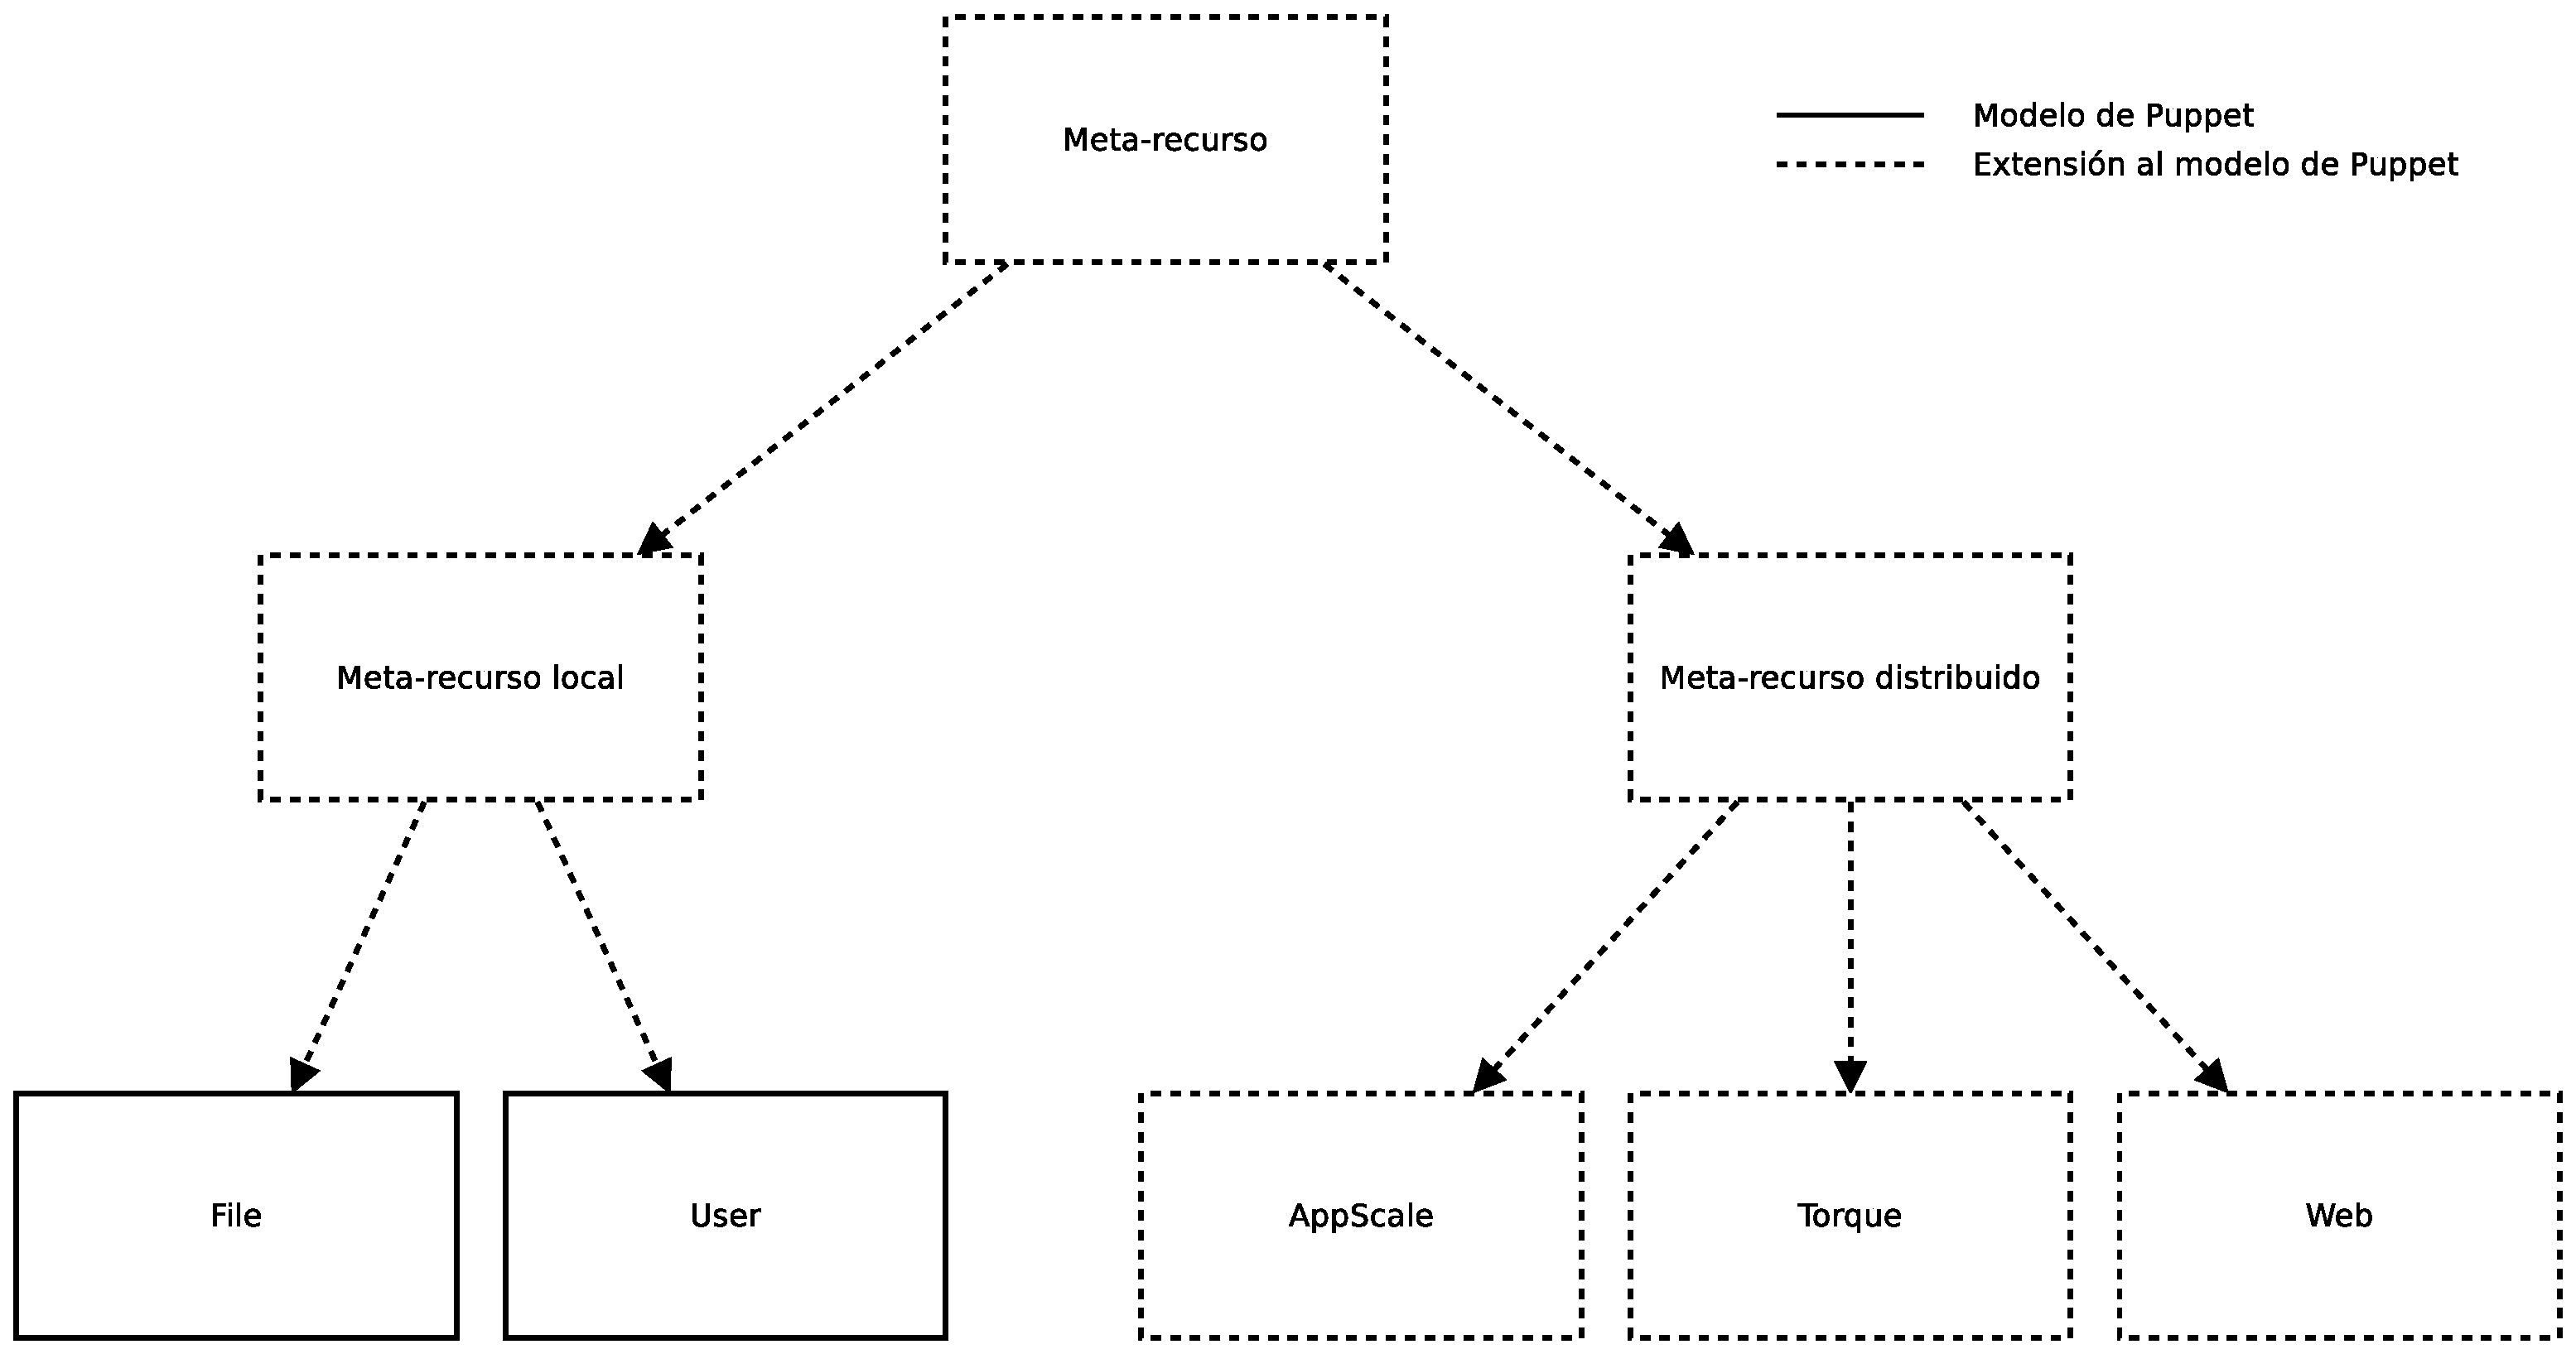
\includegraphics[width=\textwidth]{figuras/Modelo_Teorico_Puppet.eps}
  \caption{Modelado teórico de recursos en Puppet.}
\label{figure:puppet-modelo-teorico}
\end{figure}

%%% Revisar
% Se puede hacer una analogía con la programación orientada a objetos en la que el recurso distribuido sería una metaclase que proporcionaría los atributos y métodos comunes a todo recurso distribuido tales como un nombre o una administración básica. La instanciación de ese recurso en un recurso distribuido de tipo AppScale, Torque, web u otros sería similar a la instanciación de una clase a partir de la metaclase. De igual manera, el recurso distribuido instanciado podría añadir nuevos atributos y métodos y modificar el comportamiento de los métodos de la metaclase, ya que no tienen por qué iniciarse de igual manera el recurso AppScale y el recurso Torque.\\

%%% Revisar
% En Puppet cualquier recurso que se define se presupone definido dentro de un ámbito local. Para poder diferenciar los recursos distribuidos de los locales, se ha añadido (al final no) a la gramática de Puppet una palabra reservada. Ya que los ejemplos caen dentro de la categoría de \emph{cloud} la palabra que se ha escogido ha sido \texttt{cloudres}.\\

Para modelar un recurso \emph{cloud}, se han considerado como fundamentales los siguientes parámetros:

\begin{itemize}
\item Nombre: Para identificar al \emph{cloud} de manera única.
\item Fichero de direcciones IP: Para describir qué dirección IP está asociada a cada nodo del \emph{cloud}. Como la asociación viene dada por un par <rol, dirección IP> también se le llama a este parámetro fichero de roles.
\item Fichero de imágenes de disco: Para asignar a cada nodo la correspondiente imagen de disco duro.
\item Fichero de dominio: Para definir una máquina virtual especificando sus características \emph{hardware}.
\item Conjunto de máquinas físicas: Para indicar qué máquinas físicas pueden ejecutar las máquinas virtuales definidas.
\end{itemize}

Para modelar un recurso \emph{cloud} de tipo Torque podríamos usar algo similar a:

\begin{lstlisting}
torque {'torque-cloud':
   ip_file  => "/etc/puppet/modules/torque/files/jobs-ip.yaml",
   img_file => "/etc/puppet/modules/torque/files/jobs-img.yaml",
   domain   => "/etc/puppet/modules/torque/files/mycloud-template.xml",
   pool     => ["155.210.155.70"],
   ensure   => running,
}
\end{lstlisting}


\section{Diseño del proveedor de recursos distribuidos}

Puppet puede ser extendido para incluir la definición de nuevos recursos. Para ello hay que proporcinarle, como mínimo, dos ficheros: uno en el que se define el recurso y otro en el que se define cómo gestionar ese recurso. Al fichero en el que se define el recurso se le llama tipo y al fichero en el que se define cómo gestionarlo se le llama proveedor. Es decir, el tipo se encarga del ``qué'' y el proveedor se encarga del ``cómo''.\\

En un recurso cloud la definición en el fichero tipo contendría los parámetros propios de ese tipo de cloud. En el ejemplo anterior éstos serían: \texttt{ip\_file}, \texttt{img\_file}, \texttt{domain} y \texttt{pool} (el parámetro \texttt{ensure} es común a todo recurso puppet y se define automáticamente). Una vez modelado el recurso \emph{cloud}, queda como tarea proporcionar un proveedor que se encargue de llevar el \emph{cloud} al estado que se le indique desde el manifiesto Puppet. Un \emph{cloud} podrá estar en dos estados: funcionando o parado. Si tiene que estar funcionando, el proveedor se encargará de todos los pasos necesarios para llevar al \emph{cloud} a ese estado, que a grandes rasgos son:

\begin{itemize}
\item Comprobación de la existencia del \emph{cloud}: si existe se realizarán tareas de mantenimiento, si no existe se creará.
\item Comprobación del estado del conjunto de máquinas físicas.
\item Obtención de las direcciones IP de los nodos y los roles que les han sido asignados.
\item Comprobación del estado de las máquinas virtuales: si están funcionando se monitorizan, mientras que si no están funcionando hay que definir una nueva máquina virtual y ponerla en funcionamiento. Las funciones de monitorización incluyen el envío de un fichero mediante el cual cada nodo se autoadministre la mayor parte posible.
\item Cuando todas las máquinas virtuales estén funcionando se procede a inicializar el \emph{cloud}.
\item Operaciones de puesta en marcha particulares a cada tipo de \emph{cloud}.
\end{itemize}

De la misma manera, si decidimos que el \emph{cloud} tiene que estar parado, el proveedor se encargará de realizar los pasos necesarios para ello. Estos pasos son:

\begin{itemize}
\item Comprobación de la existencia del \emph{cloud}: si existe se procederá a su parada.
\item Operaciones de parada particulares a cada tipo de \emph{cloud}.
\item Apagado y borrado de las definiciones de las máquinas virtuales creadas explícitamente para este \emph{cloud}.
\item Parada de las funciones de automantenimiento de los nodos.
\item Eliminación de los ficheros internos de gestión del \emph{cloud}.
\end{itemize}

Una parte muy importante del proveedor es el parámetro \texttt{ip\_file}. En este fichero se define una asociación entre la dirección IP del nodo y el rol que cumplirá dentro del \emph{cloud}. Siguiendo con el ejemplo del recurso \emph{cloud} de tipo Torque, el fichero de roles en el que se especifica quién es el nodo maestro y la lista de nodos de computación sería similar a este:

\begin{yamlcode}
--- 
:head: 155.210.155.73
:compute:
- 155.210.155.177
\end{yamlcode}


\section{Implementación del proveedor [Temporal]}
La primera opción que se barajó fue la de usar \emph{Faces} de Puppet. \emph{Faces} es una API para crear subcomandos y acciones dentro de Puppet. Analizada a fondo, esta API no proporcionaba una ventaja muy superior a la ejecución de comandos desde la consola del sistema operativo, y no interesaba crear una abstracción que facilitara el trabajo para posteriormente estar usando continuamente la línea de comandos.

La segunda opción que se barajó fue la de la creación de un tipo y un proveedor para ese tipo. Esta opción sí que presenta una ventaja considerable: podemos usar el tipo para modelar la infraestructura distribuida y podemos usar el proveedor para indicar cómo iniciar y mantener esa infraestructura. Esta aproximación se acerca más al modelo que usa Puppet, ya que definimos la infraestructura como si fuera un recurso más de los que posee Puppet. Así pues, esta es la aproximación que se tomó para realizar la extensión.
